\section*{Описание экспериментальной установки}

\begin{figure}[H]
	\centering
	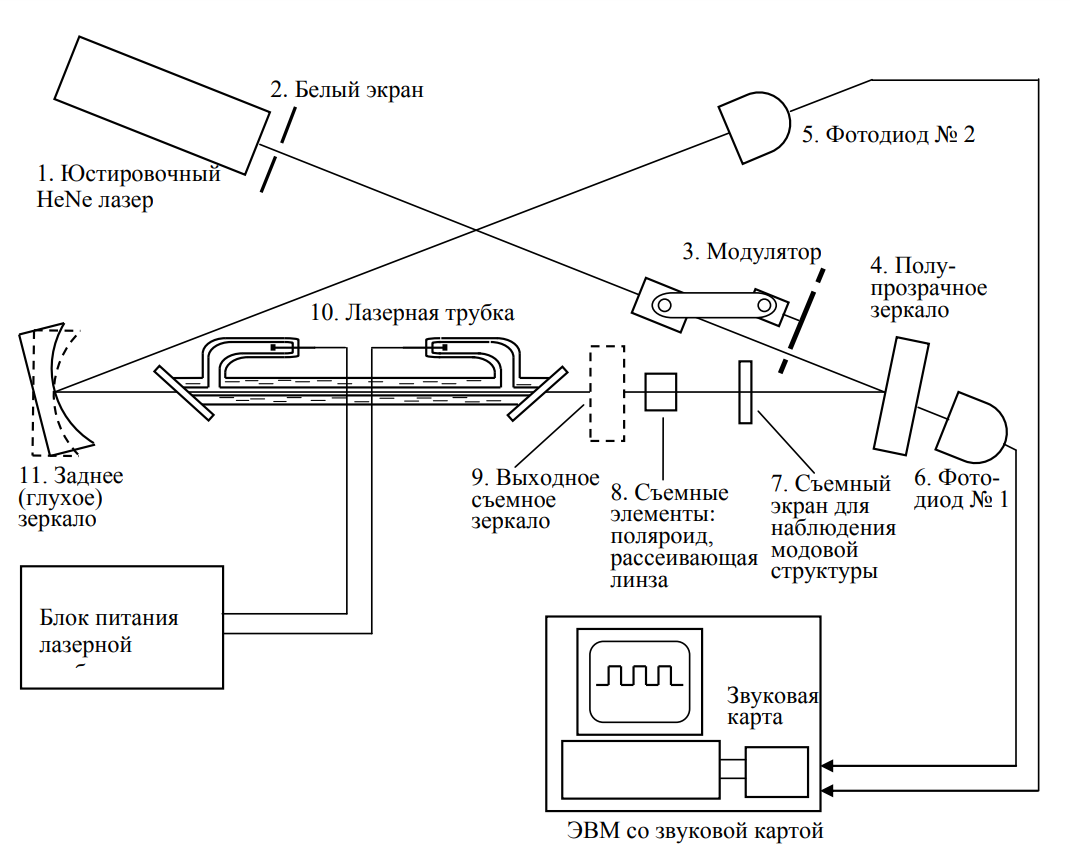
\includegraphics[width=0.7\textwidth]{../Изображения/Схема установки.png}
	\caption{Схема экспериментальной установки}
\end{figure}

На одном оптической рельсе расположены: головка промышленного Гелий-Неонового лазера ЛГ–75 с исследуемой газоразрядной трубкой (11), заключённой в кожух (10), рейтер с полупрозрачным зеркалом (4), фотодиоды (5 и 6), а также 3 съёмных рейтера с выходным зеркалом (9), отрицательной линзой для наблюдения модовой структуры излучения исследуемого лазера или поляроидом для исследования поляризации выходного излучения лазера (8) и с белым экраном (7). Юстировочный лазер (1) с белым экранчиком (2) и модулятор (3) закреплены на втором оптическом рельсе. Модулятор может быть повёрнут в разные положения: при измерении коэффициента усиления он модулирует пучок, идущий от юстировочного лазера, при измерении поляризации излучения исследуемого лазера он модулирует выходящее из него излучение. В остальных случаях модулятор отводится в сторону, чтобы не перекрывать пучки. Юстировочный лазер предназначен для настройки положения всех элементов установки и является источником зондирующего излучения для измерения усиления активной среды исследуемого лазера. Зондирующий пучок сначала попадает на полупрозрачное зеркало (4). Часть излучения проходит сквозь зеркало и попадает на фотодиод № 1 (6), с которого снимается сигнал, пропорциональный интенсивности зондирующего пучка. Отражённая часть направляется в исследуемую трубку.